\section{The CudaForge Framework for CUDA Kernel Optimization}\label{sec:proposed:approaches}
\vspace{-8pt}
\subsection{CudaForge Framework}\label{sec:overview}
 \vspace{-6pt}
Given a CUDA kernel generation task, the objective is to generate a kernel that is functionally equivalent to its PyTorch reference while achieving the lowest possible execution latency.

Inspired by the iterative workflow of human experts~\citep{10946796,cudaguide,w4a8gemm}, we design \agentname~as an iterative multi-agent framework, illustrated in Figure~\ref{fig:pipeline}.  The framework involves two independent agents: a \textbf{Coder} and a \textbf{Judge}. 
The Coder generates candidate kernels based on the task description and feedback from the Judge, while the Judge evaluates each candidate using the kernel itself, hardware feedback, and runtime information.

\begin{figure}[htbp]
  % \vspace{-4pt}
  \centering
  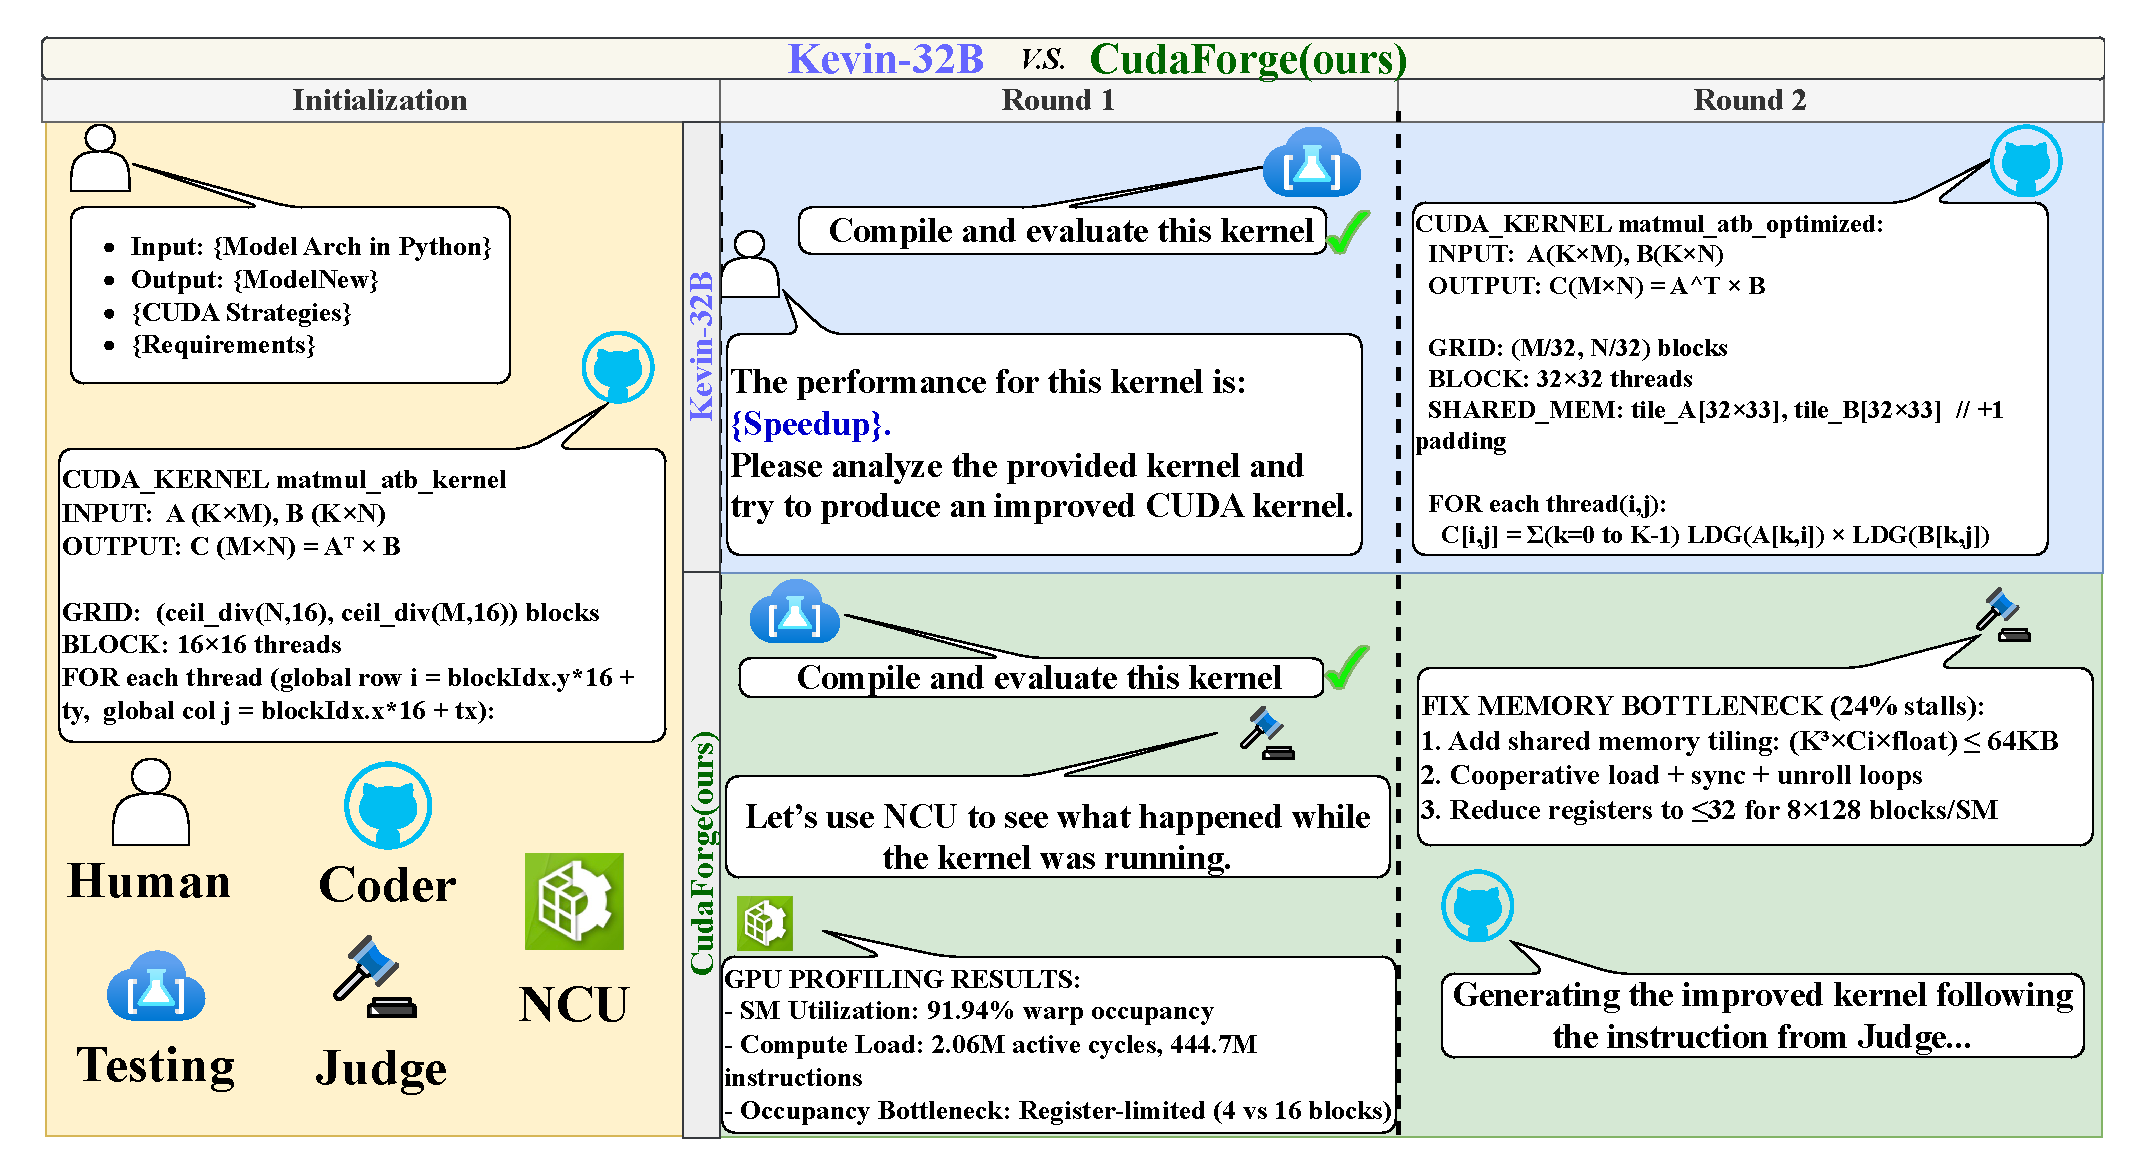
\includegraphics[width=\linewidth]{pic/pipeline_v4.pdf}
  \caption{
The overview of how \agentname~optimizes kernels, compared with Kevin-32B. 
\textbf{Top:} the pipeline of the RL-based Kevin-32B, which relies solely on textual refinement and thus performs blind exploration. 
\textbf{Bottom:} our \agentname~workflow, which leverages hardware feedback to guide kernel optimization. 
When the Coder in \agentname~generates a correct candidate kernel in Round~1, the system profiles it using Nsight Compute (NCU) to obtain NCU metrics. 
In  Round~2, the Judge analyzes these metrics and GPU specifications to identify performance bottlenecks (e.g., register- or memory-limited) and provides targeted optimization feedback. 
The Coder then refines the kernel accordingly. 
Compared with Kevin-32B, which only refines based on speedup scores, our framework achieves more interpretable and effective performance improvements through hardware-aware iteration. 
}

  \label{fig:detail}
  \vspace{-8pt}
\end{figure}
\noindent 

More specifically, given a CUDA kernel generation task, the Coder first receives the task requirements and PyTorch reference implementation, then produces an initial candidate kernel.  
This kernel is compiled and executed on test cases to check its correctness.  
If it fails, the Judge inspects {\it runtime information} (e.g. compilation errors, mismatched outputs with the PyTorch reference) and analyzes the faulty kernel. It then returns {correction feedback} (e.g. missing header file) to guide the next round. Once a kernel candidate passes the  correctness test, the Judge profiles it with the NCU tool to obtain {NCU metrics} (e.g. memory throughput, occupancy, warp efficiency).  
Together with {GPU specifications}, these metrics form the {\it hardware feedback} that allows the Judge to identify the dominant bottleneck (e.g. compute-bound or memory-bound) and provide one specific {optimization feedback} (e.g. using shared memory) to the Coder.  


In the next round, the Coder is prompted with the previous kernel, Judge feedback, and the original task requirements, and generates a corrected or optimized kernel.  
This process repeats for up to $N$ rounds, after which we select the most efficient correct kernel as the final solution.

\agentname~achieves reliability and efficiency through {\bf three key design choices}.
First, it adopts a two-agent system where the Coder focuses on generation and the Judge on evaluation, separating the “cognitive” load (See Section~\ref{Ablation-agents} for ablation study). The Coder receives only feedback from the Judge, while the Judge uses hardware and runtime information to guide generation and optimization. This division of labor mirrors human workflows and mitigates the risk of overlooking errors or inefficiencies.
Second, the framework follows an iterative optimization process, progressively correcting errors and improving efficiency across rounds. This enables stable refinement, especially on hard tasks.
Third, it explicitly incorporates hardware feedback, such as GPU specifications and NCU metrics, so that the Judge can pinpoint bottlenecks and provide actionable guidance to the Coder. This targeted optimization avoids blind exploration and ensures directed performance gains. 

\vspace{-10pt}
\subsection{Component Design}
\vspace{-4pt}
\paragraph{Design of Coder.} 
The {Coder} acts as the generative module in our framework, responsible for producing functionally correct and efficient CUDA kernel candidates given the task description, previous candidates, and feedback from the Judge. 
Directly generating a CUDA kernel from scratch is a highly challenging task for LLMs~\citep{ouyang2025kernelbenchllmswriteefficient}. 
Following the setting of KernelBench~\citep{ouyang2025kernelbenchllmswriteefficient}, we provide the Coder with a {one-shot demonstration} in the prompt, which includes an example pair of a PyTorch reference and its corresponding CUDA kernel implementation. 
This example serves as a structural and stylistic guide, helping the Coder understand the expected syntax, memory access patterns, and API usage required for valid kernel generation.

Moreover, we find that managing the Coder’s {memory scope} is crucial for stable and efficient generation. 
Prompting the model with the entire dialogue history introduces excessive context redundancy, often leading to hallucinated kernel code and higher API cost. 
To mitigate these issues, we adopt a {lightweight memory} design, where the Coder is prompted round by round without retaining the full conversation history. 
In each round, it only receives the {\it latest} feedback from the Judge, previous kernel candidate, and task description, enabling it to focus on refining or correcting the previous version. 
This design greatly improves code stability, reduces inference cost, and allows the model to perform precise, hardware-driven optimizations. See Appendix~\ref{app:prompt} for Coder's prompt.
\vspace{-8pt}
\paragraph{Design of Correctness Tests.} 
After the Coder generates a candidate kernel, our workflow proceeds to verify its {\it correctness} 
through a two-stage {testing process}, including {compilation} and {execution}. 
The compilation stage ensures that the generated kernel is syntactically valid and can be successfully compiled into executable CUDA code. 
The execution stage then evaluates the functional correctness of the compiled kernel by running it on predefined test cases. 
We compare the kernel’s outputs with those from the PyTorch reference implementation under the same inputs, and consider the kernel {functionally correct} only if the numerical difference between the two outputs is within a small tolerance (set to $1\text{e}{-4}$ in our experiments). 
A kernel is regarded as {correct} only when it passes both compilation and execution stages successfully, which is a commonly adopted criterion~\citep{kevin-multi-turn-rl,lange2025robustagenticcudakernel,ouyang2025kernelbenchllmswriteefficient}.
\vspace{-8pt}
\paragraph{Design of Judge.} 
The {Judge} serves as the evaluation and guidance module in our framework. 
Its primary responsibility is to provide actionable feedback to guide the Coder’s next round given task description, current candidate kernel, and hardware feedback or runtime information. 
The Judge operates in two distinct modes depending on kernel validity:
If the kernel fails compilation or produces incorrect outputs, the Judge performs the {\it correction mode}, identifying issues such as invalid indexing, race conditions, or missing headers, and returns \textbf{correction feedback} that instructs the Coder to fix them. 
If the kernel passes all correctness checks, the Judge enters {\it  optimization mode}, where it uses hardware feedback  to identify the dominant bottleneck—e.g., memory-bound, compute-bound, or occupancy-limited—and formulates \textbf{optimization feedback} accordingly. Please see Section \ref{sec:searching} for details of using hardware feedback. 

Similar to the design of the Coder, the Judge does not retain the full conversation. 
In each round, the Judge is prompted with the relevant mode and acts according to the corresponding role. Finally, it generates structured feedback in JSON format, which is then extracted and passed to the Coder for the next round. 
This design ensures modularity and clarity in the interaction between agents, allowing the Judge to efficiently translate hardware-level profiling signals into precise, interpretable feedback that drives iterative kernel optimization. See Appendix~\ref{app:prompt} for the Judge's prompt.


\vspace{-12pt}


\subsection{How to Integrate Hardware Feedback}\label{sec:searching}
\vspace{-8pt}
In this subsection,  we describe in detail a key design consideration, which enables \agentname~to utilize hardware feedback for kernel performance optimization.
The {hardware feedback} integrates static GPU specifications (e.g. architecture, memory bandwidth, per-thread register limits, per-SM shared-memory capacity) with performance metrics (e.g. memory throughput, occupancy, and warp efficiency) from {Nsight Compute (NCU)} collected during kernel execution. By cross-referencing GPU specifications and NCU metrics, the Judge infers the kernel’s primary performance-limiting cause and bottleneck. Figure~\ref {fig:detail} illustrates how Judge uses hardware feedback to optimize kernels.


Just as CUDA engineers focus on key indicators, we choose not to pass the entire set of NCU metrics to the Judge. Feeding all metrics can overwhelm the decision process with excessive, partially redundant signals and lead to unstable judgments (See Section~\ref{NCU} and Appendix~\ref {app:why_subset} for ablation study and case study). Instead, we design a novel protocol which profiles a subset of critical metrics provided by NCU and forward them to Judge so that we can improve the quality of the judge outputs. %prevent unstable judgments and unreasoning optimization comments. 
More specifically, the key subset of metrics are selected off-line (before the workflow starts to work), through the following steps: 


 \noindent{\bf (Step 1)} {\sf Kernel sampling and Selection}: We first profile key metrics on some preselected representative tasks (e.g., Conv2D, MatMul) to prepare a reliable metric set. Specifically, for each task we run 100 self-refine (repeating the cycle generating $\to$ execute/profile $\to$ evaluate $\to$ repair/optimize) with a single SOTA model (e.g. OpenAI-o3), collect the generated and correct kernels, and select $10$ with the largest speed disparity (fastest vs. slowest). See Algorithm~\ref{alg::alg1}. 
 
\begin{algorithm}[H]
\caption{Step 1: Kernel Sampling and Selection}\label{alg::alg1}
\KwIn{Task set $Task = \{T_1, T_2, \dots, T_n\}$}
\KwOut{Selected subsets $K_i^*$ for each task $T_i$}

\For{$i \gets 1$ \textbf{to} $n$}{
    $K_i \gets \emptyset$\;
    \For{$j \gets 1$ \textbf{to} $100$}{
        $k_j \gets \text{generate\_kernel}(T_i)$\;
        $K_i \gets K_i \cup \{k_j\}$\;
    }
    Sort $K_i$ in nondecreasing order according to kernel runtime\;
    $m \gets |K_i|$ \tcp*{Here $m=100$}
    $K_i^* \gets \{K_i[1], K_i[2], K_i[3], K_i[4], K_i[5], K_i[m-4], K_i[m-3], K_i[m-2], K_i[m-1], K_i[m]\}$\;
}
\end{algorithm}


  \noindent{\bf (Step 2)} {\sf Top-20 metrics within each task}: We then refine the metrics within each task to identify the most relevant candidates. Specifically, for each task we consolidate the NCU metrics from the $10$ kernels selected from Step 1 into a single dataset. Since Nsight Compute reports a consistent full set of metrics across all kernels, the metric categories are aligned by default. We then remove aliases and strongly collinear indicators, and compute Pearson correlations between each metric and kernel runtime. We retain only the Top-20 metrics (by absolute correlation) as the candidate set for this task (see Appendix~\ref{app:top-20}  for examples). 


\noindent{\bf (Step 3)} {\sf Metrics selection across tasks}: Finally, we consolidate metrics across tasks to build a stable, task-agnostic set. We compare the Top-20 lists across tasks and keep metrics that consistently appear, show the same correlation direction, and achieve high global scores. Specifically, for each metric, we compute a {\it global correlation score} defined as the average of its absolute Pearson correlations with runtime across all tasks. We then select metrics whose global scores exceed the 75th percentile ($P_{75}$) among all candidates, ensuring that only the most strongly correlated metrics are retained. This yields 24 metrics that are strongly correlated with kernel runtime across tasks. Later, the Judge will profile each generated kernel with NCU and uses only this 24 metrics as references (see Appendix~\ref{app:key24} for the complete list of the selected metrics).  See Algorithm~\ref{alg::alg2}. 


\begin{algorithm}[H]
\caption{Step 2-3: Profiling and Metrics Selection}\label{alg::alg2}
\KwIn{$K^* = \{K_1^*, K_2^*, \dots, K_n^*\}$, where each $K_i^* = \{k_1^*, k_2^*, \dots, k_{10}^*\}$}
\KwOut{Final metrics set $Final\_Metrics$}

$M^* \gets \emptyset$\;

\For{$i \gets 1$ \textbf{to} $n$}{
    $M_i^* \gets \emptyset$\;
    \ForEach{$k \in K_i^*$}{
        $M \gets \text{NCU\_Profile}(k)$ \tcp*{Run NCU profiling, $M=\{m_1, m_2, \dots, m_j\}$}
        \ForEach{$m \in M$}{
           $r_{m,i}$ = Compute Pearson correlation coefficient $r\!\left(m,\ \text{runtime}(k)\right)$\;
        }
        $Top20(k) \gets \text{the 20 metrics in } M \text{ with highest } |r(\cdot,\text{runtime}(k))|$\;
        $M_i^* \gets M_i^* \cup Top20(k)$\;
    }
    $M^* \gets M^* \cup M_i^*$\;
}
\tcp{Compute global correlation scores across tasks}
\ForEach{metric $m \in M^*$}{
    Compute $S_m = \frac{1}{n}\sum_{i=1}^{n} |r_{m,i}|$  
    \tcp*{$r_{m,i}$: Pearson correlation between metric $m$ and runtime on task $i$}
}

\tcp{Select stable and highly correlated metrics}
$Final\_Metrics \gets \{m \mid m \text{ appears in multiple tasks, keeps same sign, and } S_m > P_{75}(S)\}$\;



\tcp{Final set contains 24 distinct metrics}
\end{algorithm}



After the key subset of NCU metrics is determined offline, the Judge will use these metrics to identify performance bottlenecks in the \agentname~workflow. At each optimization round, the Judge profiles the generated kernel with NCU and collects hardware feedback, including static GPU specifications and the key subset of NCU metrics.  Based on this information, the Judge identifies the dominant bottleneck in the current kernel. 
To prevent AI agent reasoning without direction and generating suboptimal results, the Judge is prompted to only capture 3-4 most important metrics in each round according to its own reasoning. For example, Judge can identify the current kernel as memory-bound when memory throughput is high but computing resource utilization is low, and then it will choose memory related metrics as critical metrics in this round. After this, Judge will generate suggestions on how to modify the kernel to address the current critical bottleneck. The Coder incorporates this guidance in the next round generation accordingly. This mechanism enables our multi-agent system focus on addressing only one critical program bottleneck in each round, and eventually optimizes overall kernel performance step by step in iterative rounds, just like human experts' real workflow. 


